\section{Taylor-Green vortex}
A more sophisticated system than the Poisseuille flow is the decaying
Taylor-Green vortex flow. Also this system is one of the few where an
analytical solution to Navier-Stokes is possible to find. In this
section, the Taylor-Green flow is used to benchmark the 2D LBM
proposed in section \ref{sec:lbm:ns}. The force implementation is also
tested in 2D in section \ref{sec:mb:four_rows}. 

The Taylor-Green vortex flow in two dimensions is defined by the
following pressure and velocity fields \cite{junk-asym}:

\begin{equation}\label{eq:mb:tv}
\begin{aligned}
u_x(\x, t) &= -\frac{1}{a}\cos(ax)\sin(by)\exp(-\nu(a^2 +
b^2)t)\\ 
u_y(\x, t) &= \frac{1}{b}\sin(ax)\cos(by)\exp(-\nu(a^2 +
b^2)t)\\ 
P(\x, t) &= -\frac{1}{4} \left( \frac{1}{a^2}\cos(2ax) +
\frac{1}{b^2}\cos(2by)\right) \exp(-2\nu(a^2 + b^2)t)
\end{aligned}
\end{equation}
where $\nu$ is the viscosity, $\x\in[0, 2\pi]^2$ and $a$ and $b$ are
two real constants. It is straight-forward to verify that these
quantities satisfy the incompressible Navier-Stokes,
eqs. \eqref{eq:et:ns_incompressible} and \eqref{eq:et:ns_mom}. The
constants $a$ and $b$ is chosen as $a = b = 2\pi/N$ where $N = N_x =
N_y = 100$ is the grid resolution. This particular choice of $a$ and
$b$ allows us to use lattice units with $\delta_x = \delta_t = 1$ in
the simulation. The maximum velocity in the vortex at $t_0$ is chosen
as $u_0 = 1/a = 1/b$.

The simulation is performed with $\nu = 0.05$ l.u. on a $100\times100$
lattice. Following the initialisation with the analytical solution,
eq. \eqref{eq:mb:tv}, at $t = 0$, the decay is studied and compared
with the analytical solution. Initialisation of the velocities is done
by setting $\fii = \feq(\rho, \ubf)$ where $\rho$ includes both the
constant density (order $\ep^0$) and the pressure (order $\ep^2$),
compare eq. \eqref{eq:lbm:ns_mom_index}.

The result is presented in fig. \ref{fig:mb:taylor_vis} where the
velocity field and the magnitude of the velocity field is
visualised. This is at a time, $t_{1/2}$, where the maximum magnitude
of the velocity has decreased to half of the initial value,
i.e. $t_{1/2} = \log(2)/(2\nu(2\pi/N)^2)$. In
fig. \ref{fig:mb:taylor_vis}, the analytical and the computed
solutions is compared on a section of the domain at $t = t_{1/2}$. The
agreement with an average error in the order of $10^{-3}$ is
comparable with previous works, e.g. \cite{junk-asym}.


\begin{figure}
  \centering
  \subfloat[Velocity field
    ]{\label{fig:mb:t1}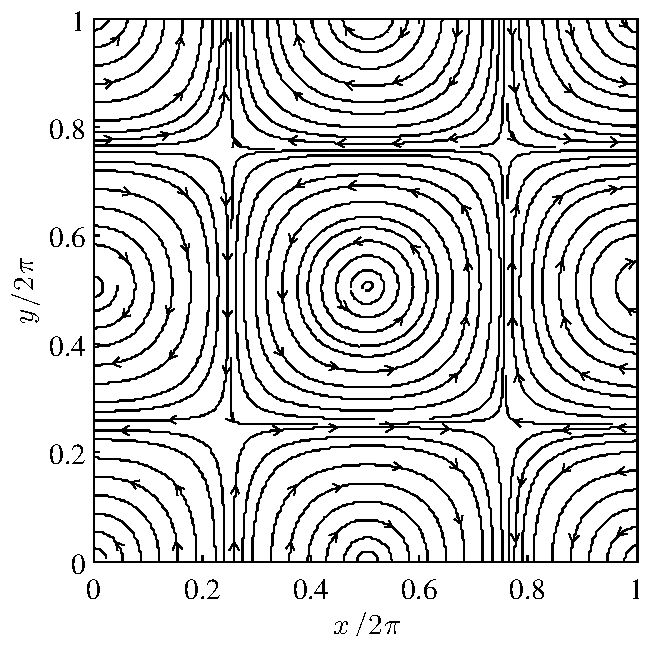
\includegraphics[width=0.47\textwidth]{fig/tg_vortex.pdf}}      
  \hspace{5pt} \subfloat[$|\ubf|$
  ]{\label{fig:mb:t2}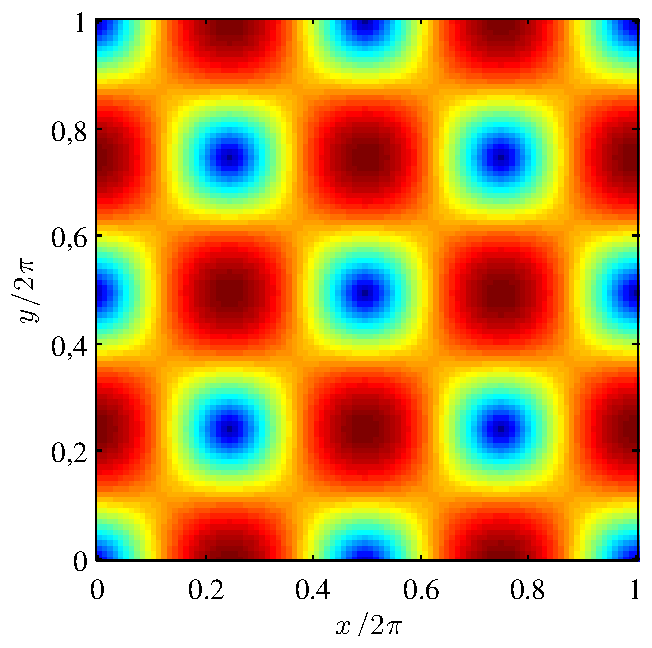
\includegraphics[width=0.47\textwidth]{fig/tg_u.pdf}}
  \caption{Visualised velocity field (a) and magnitude of the
    velocities (b) for a decaying Taylor-Green vortex. The velocity
    field is taken at $t=t_{1/2}$ and the values in (b) varies from
    $-u_0/2$ (blue) to $u_0/2$ (red).}
  \label{fig:mb:taylor_vis}
\end{figure}

\begin{figure}
\begin{center}
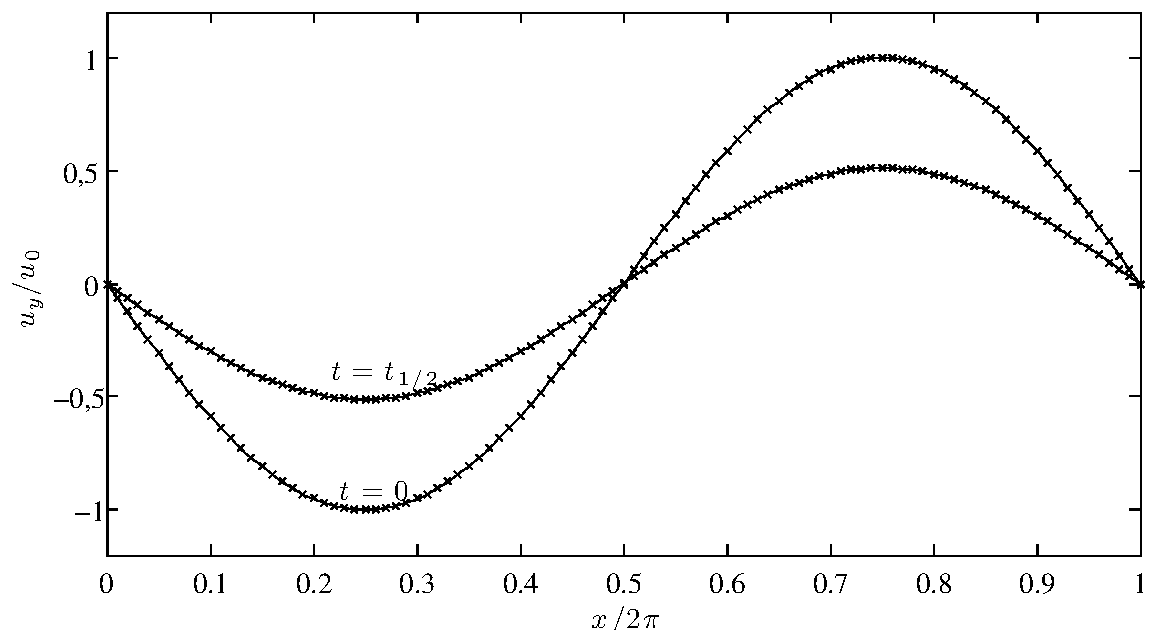
\includegraphics[width=0.9\textwidth]{fig/taylor_uy.pdf}
\end{center}
\caption{1D section of the decaying Taylor-Green flow. The $y$
  component of the velocity is plotted at $y = \pi$. Computed solutions
  ($\times$) are compared with analytical (solid) at two different
  times $t = t_0$ and $t = t_{1/2}$. A domain of $100\times100$ nodes
  were used.}
\label{fig:mb:tg_uy}
\end{figure}

\subsection{Four rows mill}\label{sec:mb:four_rows}
In the decaying Taylor-Green case, the time derivative term in
Navier-Stokes momentum equation is balanced by the viscous term. We
now wish to compensate for the decay by introducing a force. In a
steady state situation, $\partial_t\ubf = 0$ and the force must
balance the viscous term. The force is therefore chosen as

\begin{equation}
\begin{aligned}
F_x(\x, t) &= \nu(a^2 + b^2)u_x(\x, t) \\
F_y(\x, t) &= \nu(a^2 + b^2)u_y(\x, t) 
\end{aligned}
\end{equation}
where $u_x$ and $u_y$ are velocities from eq. \eqref{eq:mb:tv}. Using
the same parameters, initialisation and domain as in the decaying
case, no decay is observed. In fig. \ref{fig:mb:four_mill}, a section
of the $y$ component of the velocity is shown at $t = t_{1/2}$.

\begin{figure}
\begin{center}
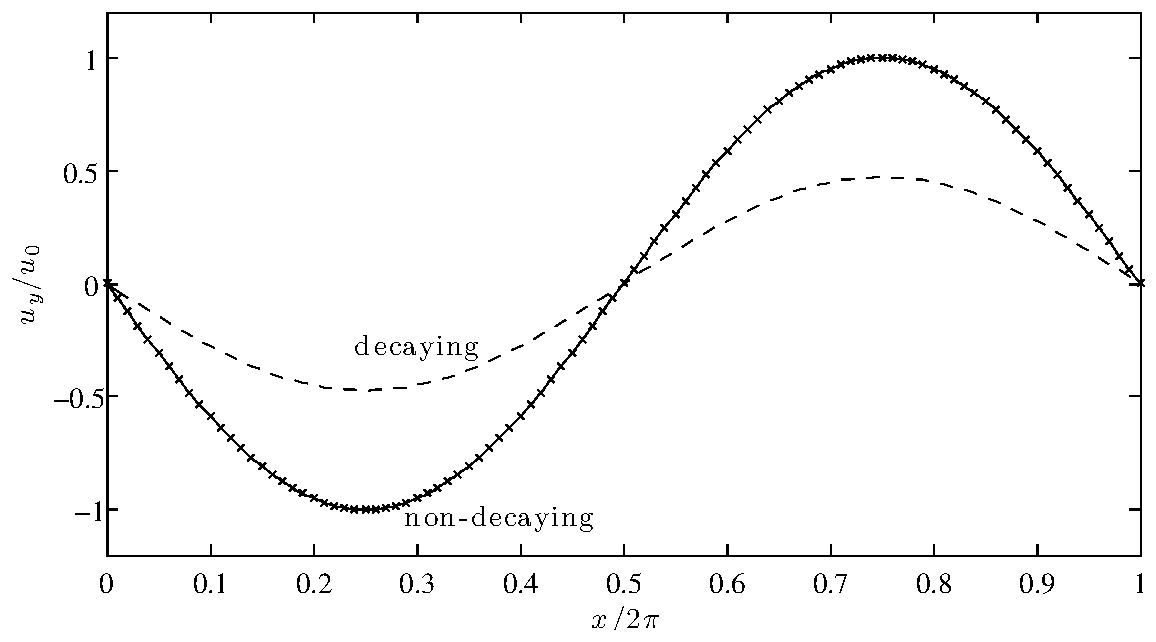
\includegraphics[width=0.9\textwidth]{fig/four_mill.pdf}
\end{center}
\caption{1D section of the steady four rows mills flow at $t =
  t_{1/2}$. An external force have been included to compensate the
  decay (dashed). The $y$ component is plotted for $y = \pi$. }
\label{fig:mb:four_mill}
\end{figure}

